\documentclass[11pt]{article}
\setlength{\textwidth}{6in}
\setlength{\textheight}{9in}
\setlength{\evensidemargin}{0in}
\setlength{\oddsidemargin}{0in}
\setlength{\footskip}{.5in}
\setlength{\topmargin}{0in}
\setlength{\parskip}{6pt plus 2pt minus 1pt}
\renewcommand{\thesection}{\arabic{section}.}

\usepackage{nopageno,url,natbib}
\usepackage{graphicx, amsmath, amssymb, hyperref,caption,subcaption}
\usepackage[hang,flushmargin]{footmisc}
\usepackage{xcolor}
\hypersetup{
    colorlinks,
    linkcolor={red!50!black},
    citecolor={blue!50!black},
    urlcolor={blue!80!black}
}

% Prep-reading / interactive links (defined once, reused throughout)
\newcommand{\chmdp}{\href{https://josephausterweil.github.io/probintro/intro2/21_markov_decision_processes/}{Ch~21 (Markov Decision Processes)}}
\newcommand{\chql}{\href{https://josephausterweil.github.io/probintro/intro2/22_q_learning/}{Ch~22 (Q-Learning)}}
\newcommand{\qlwidget}{\href{https://josephausterweil.github.io/probintro/widgets/qlearning-gridworld.html}{interactive $Q$-learning widget}}

\begin{document}
\begin{centering}
{\large \bf Assignment 4: Reinforcement Learning \\ Human and Machine Learning \\ Chiba Institute of Technology, School of Design \& Science \\ Prof. Joseph Austerweil \\ Due Fri Jul 10, 2026 at 8:00pm\\}
\end{centering}

In this problem set you will implement the reinforcement-learning algorithm
{\em $Q$-learning}, and then use it to see one of the central lessons of RL: an
agent optimizes the {\em reward you write}, which is not always the {\em goal you
meant}. We work in the ``GardenPath'' domain \citep*{ho15}. The goal of the domain
is to teach an agent to reach the top-right square (the ``goal'') by moving along
the left-most and top-most squares (the ``path'') while avoiding the bottom-right
$2\times2$ block (the ``garden''). Figure~\ref{fig:gardenpath} shows the domain.
A person sees the picture, but the learning algorithm only knows that there is a
$3\times3$ world it can move around in, receiving feedback as it goes.

\begin{figure}[h]
\centerline{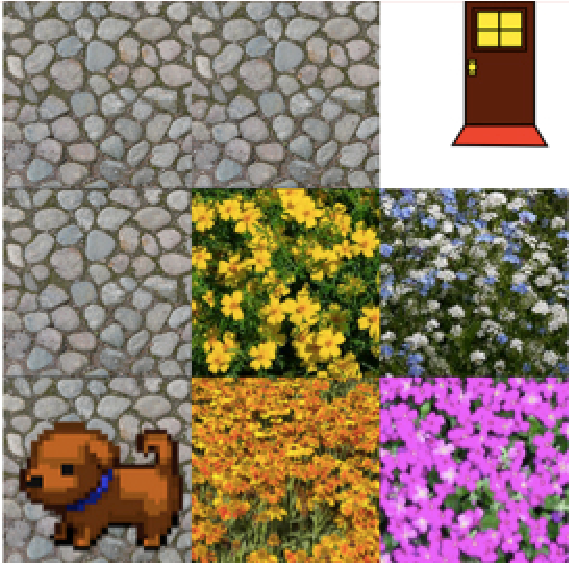
\includegraphics[width=2.6in]{figs/gardenpath}}
\caption{The GardenPath domain. Agents learn to reach the goal by moving along the path and avoiding the garden.}
\label{fig:gardenpath}
\end{figure}

\noindent The goal of reinforcement learning is to learn a {\em policy}
$\pi: S \rightarrow A$ telling the agent which action $a \in A$ to take in each
state $s \in S$ so as to maximize its reward. $Q$-learning does this by learning a
matrix $Q$ that stores the expected future reward of taking an action in a state.
It is guaranteed to find the optimal policy for a Markov decision process. The
algorithm is:
\begin{enumerate}
\item[1.] Initialize a $|S| \times |A|$ matrix $Q$ to some value (usually zero).
\item[2.] For each training episode, start at the initial state and set $t=1$.
\begin{enumerate}
\item[2a.] Select an action with an $\epsilon$-greedy rule: with probability
$1-\epsilon$ pick a best action in the current state according to $Q$ (break ties
at random), and with probability $\epsilon$ pick a random valid action.
\item[2b.] Take that action, move to a new state $s_{t+1}$, and receive feedback $f_{t+1}$.
\item[2c.] With learning rate $\alpha$ and discount factor $\gamma$, update $Q$:
\begin{equation}
Q(s_t,a_t) \;\leftarrow\; Q(s_t,a_t) + \alpha \Big(\underbrace{f_{t+1} + \gamma \max_a Q(s_{t+1}, a) - Q(s_t,a_t)}_{\text{prediction error}} \Big)
\label{eq:qlearn}
\end{equation}
\end{enumerate}
\end{enumerate}
Intuitively, the update moves $Q(s_t,a_t)$ toward the reward just received plus the
best reward expected from there on.

\paragraph{Two ways to give feedback.} The point of the assignment is to compare
two feedback schemes on this domain \citep*{ho15}.
\begin{itemize}
\item {\bf Reward-maximizing (RM)} --- {\em outcome-based} feedback: moving into
the garden is punished ($-10$), reaching the goal pays $+20$, and ordinary moves
along the path are neutral ($0$). This is the reward you would write if you cared
only about the outcome.
\item {\bf Action-feedback (AF)} --- the way {\em people} tend to teach: forward
progress along the path is praised ($+10$), and --- being encouraging --- {\em
backtracking} along the path earns faint praise ($+4$) rather than punishment.
Both directions are positive.
\end{itemize}
You can also experiment with both schemes, step by step, in the \qlwidget{} from
textbook \chql{} (it uses this exact GardenPath world).

\vspace{1em}
\noindent {\bf Stencils.} Three starter stencils are provided in this directory;
pick one and submit your completed version. Each ships with a shared helper,
\texttt{rl\_gridworld.py} (the world, the reward schemes, the figure renderer, and
an in-notebook interactive explorer); keep it next to your notebook.
\begin{itemize}
    \item \texttt{rl\_genjax.ipynb} --- GenJAX (canonical, runs in Google Colab). The environment is written as a \texttt{@gen} generative model and $Q$-learning learns by {\em sampling} it.
    \item \texttt{rl\_python.ipynb} --- numpy + matplotlib (Python without GenJAX).
    \item \texttt{rl\_nosoln.Rmd} --- base R + ggplot2 (self-contained; static figures).
\end{itemize}
A Matlab stencil is available on request --- email Prof. Austerweil.

\vspace{0.5em}
\noindent {\bf Prep reading.} Textbook Tutorial~3 --- \chmdp{} and \chql{} --- which
walk through everything this assignment asks you to implement. Both chapters embed
the \qlwidget{} (open it fullscreen to play with $\alpha$, $\gamma$, $\epsilon$ and
the feedback schemes). This assignment uses the same GardenPath world and the same
figures, so the chapters are the fastest way in.

\section{Implement $Q$-learning}
In your stencil, fill in the one-line {\em prediction error} from
Equation~\eqref{eq:qlearn} (the term under the brace; \chql{} steps through it one
stage at a time if you want to see each piece). All the setup --- the world,
$\epsilon$-greedy selection, the training loop, and the figures --- is provided.

Then train under {\bf reward-maximizing (RM)} feedback and visualize the learned
policy with the provided renderer (it draws, for each cell, the four action-values
as green/red wedges, the greedy policy as arrows, and the route the greedy policy
takes from the start). {\em Deliverable:} include the RM figure and a sentence ---
does the learned policy reach the goal, and does it make sense?

\section{Diagnose a reward-hacking failure}
Now train under {\bf action-feedback (AF)} feedback and visualize the learned
policy. {\em Deliverable:} the AF figure, the {\bf net reward per lap} of the loop
(the renderer / \texttt{greedy\_rollout} reports it), and a few sentences:
\begin{enumerate}
\item[(a)] Does the learned greedy policy reach the goal? If not, what does it do?
\item[(b)] Why does a reward-maximizing agent prefer to farm that positive cycle
forever rather than collect the one-time $+20$ at the goal?
\item[(c)] What does this show about the relationship between the reward you write
and the goal you intend? (This phenomenon is called {\em reward hacking} or {\em
specification gaming}.)
\end{enumerate}
\chql{}'s ``Reward Shaping and Positive Cycles'' section discusses this failure if
you want to compare your findings.

\section{Design and verify a fix}
AF tried to give helpful per-step feedback but accidentally created a reward cycle.
The principled way to add dense feedback is {\em potential-based shaping}
\citep*{ng99}: choose a {\bf potential} $\Phi(s)$ (a rough ``how good is this
state'') and add a potential {\em difference} to the true (RM) reward,
\begin{equation}
r'(s,a) \;=\; r_{\text{RM}}(s,a) \;+\; \gamma\,\Phi(s') - \Phi(s).
\label{eq:shaping}
\end{equation}
Because it is a {\em difference} of potentials, a step toward the goal earns a bonus
and a step away pays an equal penalty --- so there is no farmable cycle.

\begin{enumerate}
\item[(a)] {\em Design.} Choose your own potential $\Phi(s)$ (a good default is the
negative distance to the goal, so states nearer home have higher potential --- but
try your own and justify it). Build the shaped reward~\eqref{eq:shaping}, train, and
visualize. {\em Deliverable:} the figure --- does it now reach the goal?
\item[(b)] {\em Verify it is safe (invariance).} Shaping should fix learning {\em
without} changing which policy is optimal. Using the provided value-iteration
helper, compute the exact optimal policy for RM and for shaped-RM and confirm they
are identical.
\item[(c)] {\em Explain.} In a few sentences, explain why $\gamma\Phi(s')-\Phi(s)$
cannot change the optimal policy (hint: sum it along a trajectory --- what
telescopes?), and contrast this with AF: both add dense feedback, but only one
changed the optimum. Why?
\end{enumerate}

\section*{Bonus (+5)}
$Q$-learning is {\em model-free} --- it never sees the transition rules, it learns
only from samples. If we {\em know} the model (\chmdp{}), we can compute the
optimal policy exactly with {\em value iteration}. Using the provided helper,
confirm your model-free learner found the same route to the goal that the
model-based planner computes exactly. (In the GenJAX stencil, the value-iteration
step reads the same \texttt{@gen} transition model you sampled to learn.)

\vspace{0.5em}
\noindent {\bf Submission.} Submit by DM or email to the instructor {\em one} of
the following:
\begin{itemize}
    \item your completed notebook (or knitted \texttt{.Rmd}) --- it must run end-to-end and contain your figures, inline text answers, and descriptions; {\em or}
    \item a single PDF report containing your code, figures, text answers, and descriptions.
\end{itemize}

\bibliographystyle{myapalike}
\bibliography{rl}

\end{document}
